\subsection{UC11 - Annullamento Operazione }
\begin{itemize}
	\item \textbf{Identificativo}: UC11
	\item \textbf{Nome}: Annullamento Operazione
  \item \textbf{Descrizione grafica}:
\end{itemize}

\begin{figure}[h]
    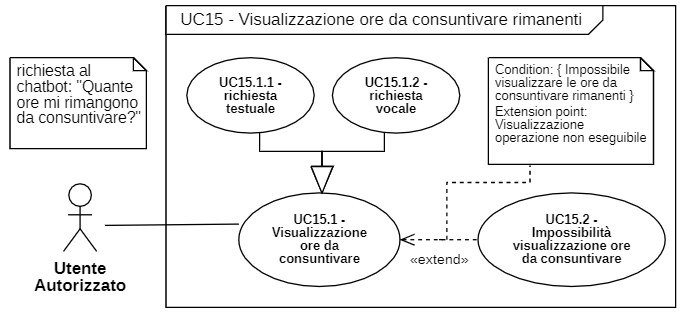
\includegraphics[scale=1.20]{images/UC11.png} 
    \caption{Descrizione grafica caso d'uso UC11}
\end{figure}
\begin{itemize}
	\item \textbf{Attori}
	\begin{itemize} 
		\item \textit{Primari}: Utente autorizzato
		\item \textit{Secondari}: Non presenti
	\end{itemize}
	\item \textbf{Descrizione}: L'utente vuole cancellare esecuzione di un'operazione precedentemente richiesta.
	\item \textbf{Precondizione}: L'utente ha richiesto un'operazione.
	\item \textbf{Postcondizione}: Operazione non viene eseguita.
	\item \textbf{Scenario principale}: \begin{enumerate}
		\item Utente comunica al chatbot: "Annulla operazione";
		\item Chatbot comunica: "Operazione annullata con successo".
	\end{enumerate}
  \item \textbf{Estensione}: L'operazione di annullamento non può essere eseguita. (UC11.2)
\end{itemize}

\paragraph{UC11.1.1 - Richiesta Testuale}
\begin{itemize}
   \item \textbf{Identificativo}: UC11.1.1
   \item \textbf{Nome}: Richiesta testuale
   \item \textbf{Descrizione grafica}: (approfondita in UC11)
   \item \textbf{Attori}:
   \begin{itemize} 
       \item \textit{Primari}: utente autorizzato
       \item \textit{Secondari}: non presenti
   \end{itemize}
       \item \textbf{Precondizione}: L'utente ha richiesto un'operazione.
       \item \textbf{Postcondizione}: Operazione non viene eseguita. 
    \item \textbf{Scenario principale}: 
       \begin{itemize}
        \item Utente scrive al chatbot: "Annulla operazione";
        \item Chatbot risponde: "Operazione annullata con successo".
       \end{itemize}
\end{itemize}

\paragraph{UC11.1.2 - Richiesta Vocale}
\begin{itemize}
   \item \textbf{Identificativo}: UC11.1.2
   \item \textbf{Nome}: Richiesta testuale
   \item \textbf{Descrizione grafica}: (approfondita in UC1)
   \item \textbf{Attori}:
   \begin{itemize} 
       \item \textit{Primari}: utente autorizzato
       \item \textit{Secondari}: non presenti
   \end{itemize}
       \item \textbf{Precondizione}: L'utente ha richiesto un'operazione.
       \item \textbf{Postcondizione}: Operazione non viene eseguita. 
    \item \textbf{Scenario principale}: 
       \begin{itemize}
        \item Utente comunica vocalmente al chatbot: "Annulla operazione";
        \item Chatbot comunica: "Operazione annullata con successo".
       \end{itemize}
\end{itemize}

\subsubsection{UC11.2 - Errore Annullamento Operazione}
\begin{itemize}
	\item \textbf{Identificativo}: UC11.2
	\item \textbf{Nome}: Errore Annullamento Operazione 
	\item \textbf{Attori}
	\begin{itemize} 
		\item \textit{Primari}: Utente autorizzato
		\item \textit{Secondari}: Non presenti
	\end{itemize}
	\item \textbf{Descrizione}: L'utente vuole annullare un'operazione.
	\item \textbf{Precondizione}: L'utente richiede di annullare un'operazione.
	\item \textbf{Postcondizione}: Viene visualizzato un errore di impossibilità di annullare l'operazione.
	\item \textbf{Scenario principale}: Utente comunica la volontà di annullare un'operazione ma questa viene negata.
\end{itemize}